\documentclass{beamer}

\usepackage{default}
\usepackage{graphicx}
\usepackage[utf8x]{inputenc}
\usepackage{amsmath}
\usepackage{amsfonts}
\usepackage{amssymb}
\usepackage{geometry}
%\usepackage{movie15}
\usepackage{media9}
%\usepackage{subfigure}
\usepackage{graphicx}
\usepackage{comment}
\usepackage{textpos}
\usepackage[spanish,es-nodecimaldot]{babel}
\usepackage{chemmacros}
\chemsetup{
formula = chemformula,
modules = thermodynamics,
modules = reactions
}
\usepackage{pict2e}
\usepackage{epstopdf}
\newcommand{\gnuplotexe}{/opt/local/bin/gnuplot}
\usepackage[shell]{gnuplottex}
\usepackage{verbatim}
\usepackage{listings}
\lstset{language=C++%
,basicstyle=\tiny\ttfamily%
,backgroundcolor=\color{black!20}%
,breaklines=true%
,keywordstyle=\bfseries\color{magenta!90}%
,commentstyle=\itshape\color{green!40!black}%
,identifierstyle=\color{black}%
,deletekeywords={for, and, not,}%
,stringstyle=\color{red!95!black}%
,numbers=left%
,numberstyle=\tiny%
,identifierstyle=\color{black}%
%,title=\lstname%
}
%%%%%%%%%%%%%%%%%%%%%%%%%%%%%%%%%%%%%%%%%%%%%%%%%%%%%%%
%%%%%%%%%%%%%%%%%%%%%%%%%%%%%%%%%%%%%%%%%%%%%%%%%%%%%%%
%%%%%%%%%%%%%%%%%%%%%%%%%%%%%%%%%%%%%%%%%%%%%%%%%%%%%%%
\newcommand{\currentWeek}{00}
%%%%%%%%%%%%%%%%%%%%%%%%%%%%%%%%%%%%%%%%%%%%%%%%%%%%%%%
%%%%%%%%%%%%%%%%%%%%%%%%%%%%%%%%%%%%%%%%%%%%%%%%%%%%%%%
%%%%%%%%%%%%%%%%%%%%%%%%%%%%%%%%%%%%%%%%%%%%%%%%%%%%%%%
\usetheme{Ilmenau}

\titlegraphic{\begin{textblock}{3}(-0.9,-4.0)
     \includegraphics[height=2.0cm, width=2.0cm]{images/buap02}
   \end{textblock}
     \begin{textblock}{3}(11.4,-4.0)
     \includegraphics[height=2.0cm, width=2.0cm]{images/fcq}
   \end{textblock}}
	\title[FCQ-BUAP]{Desarollo de software científico para el cálculo especializado de entalpías de formación}
	\author[Édgar García Juárez]
{
\textbf{T  E  S  I  S}
}
\institute[]
{  
  	Para obtener el grado de Licenciado en Química\\[0.3cm]
  	Presenta: \\
 	 \textbf{Édgar García Juárez} \\[0.5cm]
 	 Director y Asesor:\\
	\textbf{Dr. Juan Manuel Solano Altamirano}\\ 
	\textbf{Dr. Julio Manuel Hernández Pérez}\\ 
}
	\date{27 de octubre de 2022}



\begin{document}
\setbeamertemplate{page number in head/foot}[totalframenumber]
\setbeamertemplate{navigation symbols}{}
\frame{
\titlepage
}
\frame{\tableofcontents}

%*************************************************************
\section{Introducción}
%*************************************************************
%++++++++++++++++++++++++++++++++++++++++++++++++++++++++
\begin{frame}[fragile]
\frametitle{Química computacional}
Las simulaciones efectuadas por computadoras tienen múltiples ventajas:
	\vspace{1cm}
	\begin{itemize}
\item Son más ecónomicas que los experimentos físicos.
\item Pueden resolver múltiples problemas.
	\end{itemize}
\end{frame}

%...................................................
%++++++++++++++++++++++++++++++++++++++++++++++++++++++++
%++++++++++++++++++++++++++++++++++++++++++++++++++++++++
%...................................................
\begin{frame}[fragile]
\frametitle{Importancia de las funciones termodinámicas}

A la energía involucrada en una reacción química que relaciona la formación de 1 mol de un compuesto a partir de sus elementos en su forma más estable a $p$ = 1 bar y una temperaratura dada, se le conoce como \textbf{entalpía de formación}.

\end{frame}

\begin{comment}

\end{comment}

%...................................................
%++++++++++++++++++++++++++++++++++++++++++++++++++++++++
%++++++++++++++++++++++++++++++++++++++++++++++++++++++++
%...................................................
\begin{frame}[fragile]
\frametitle{Calorimentría y cálculos \textit{ab initio}}

\begin{figure}
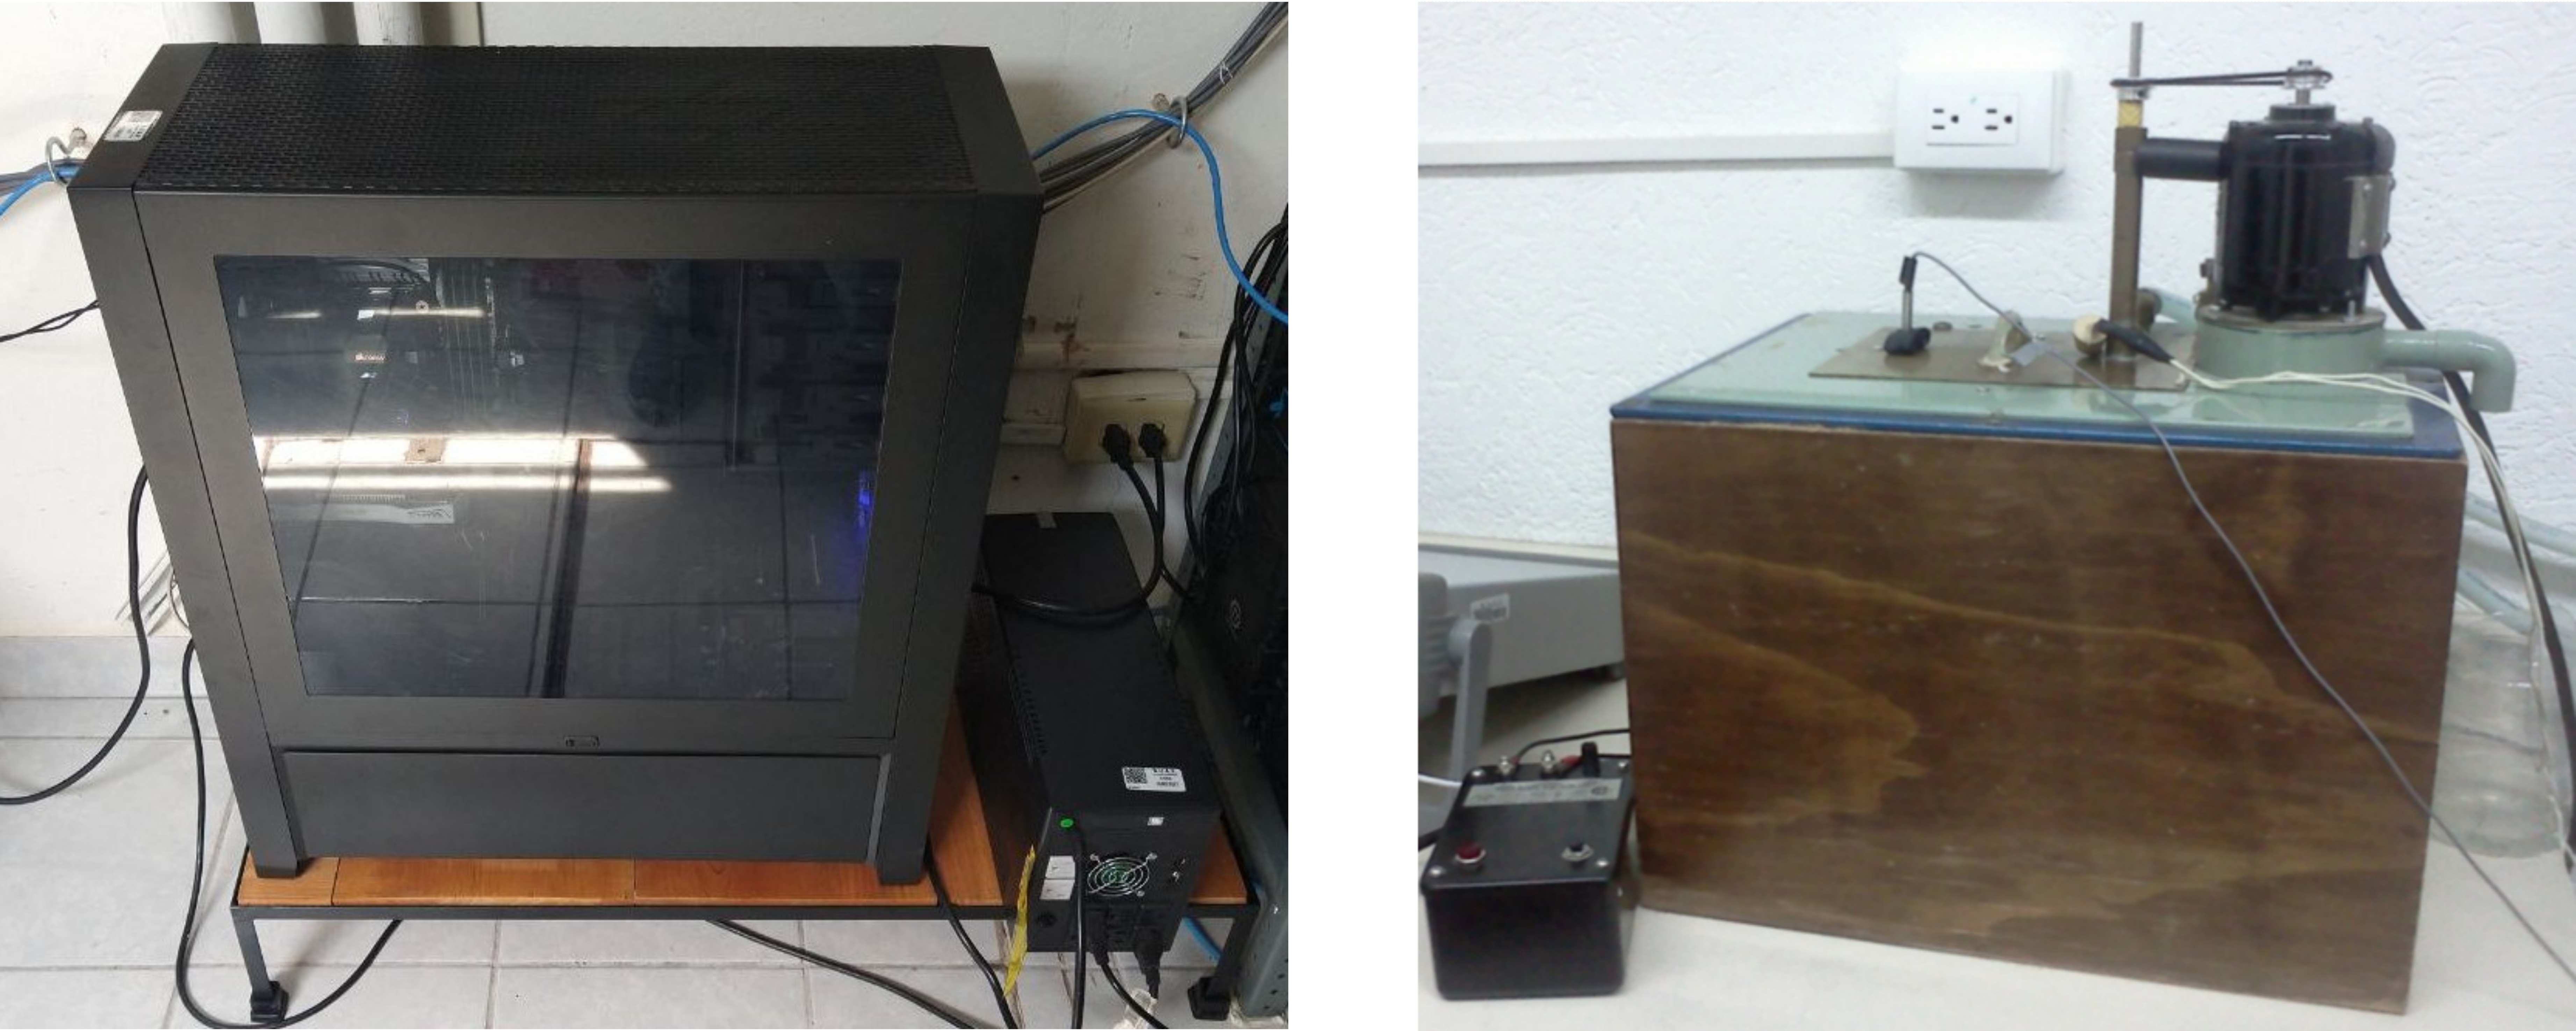
\includegraphics[height=5.0cm, width=11cm]{images/CB.png}
\caption{Servidor de cómputo y calorímetro de combustión.}
\end{figure}
\end{frame}
%...................................................
%++++++++++++++++++++++++++++++++++++++++++++++++++++++++
%++++++++++++++++++++++++++++++++++++++++++++++++++++++++
%...................................................

\begin{frame}[fragile]
\begin{figure}
\includegraphics[scale=.7]{images/PC.png}
\caption{John Pople y Larry Curtiss.}
\end{figure}
\end{frame}
%...................................................
%++++++++++++++++++++++++++++++++++++++++++++++++++++++++
%++++++++++++++++++++++++++++++++++++++++++++++++++++++++
%...................................................
\begin{frame}[fragile]
\frametitle{Método de atomización}
\begin{figure}
\includegraphics[scale=.5]{images/atomization-CH3OH}
\end{figure}
\tiny{\textit{Errol Lewars. Computational chemistry: introduction to the theory and applications of molecular and quantum mechanics. Springer, 2016.}}
\end{frame}
%...................................................
%++++++++++++++++++++++++++++++++++++++++++++++++++++++++
%++++++++++++++++++++++++++++++++++++++++++++++++++++++++
%...................................................
\begin{frame}[fragile]
\frametitle{Termodinámica estadística}

\begin{equation}
H(T)-H(0) = \int_{0} ^{T} C_{p} dT = \frac{RT^{2}}{Q} \frac{\partial Q}{\partial T} + RT
\label{eq:3.26}
\end{equation}


%\begin{equation}
%Q = Q_{tras}Q_{rot}Q_{vib}Q_{elec}
%\label{eq:3.27}
%\end{equation}

\begin{equation}
[H(T)-H(0)]_{tras} = \mathrm{\frac{3}{2}} RT
\label{eq:3.28}
\end{equation}

\begin{equation}
[H(T)-H(0)]_{rot} = \mathrm{\frac{3}{2}} RT
\label{eq:3.29}
\end{equation}


\begin{equation}
[H(T)-H(0)]_{rot}^{lineal} =  RT
\label{eq:3.30}
\end{equation}

\begin{equation}
[H(T)-H(0)]_{vib}=RT \sum_i \left(\frac{h\nu_i}{kT}\right)\left(\frac{e^{\frac{-h\nu_i}{kT}}}{1-e^{\frac{-h\nu_i}{kT}}}\right)
\label{eq:3.31}
\end{equation}
\end{frame}

\begin{frame}[fragile]


\begin{multline}
[H(298.15)-H(0)] =... \\... [H(T)-H(0)]_{tras}+[H(T)-H(0)]_{rot}+[H(T)-H(0)]_{vib}
\end{multline}


\begin{multline}
[H(298.15)-H(0)] =... \\... \mathrm{\frac{3}{2}} RT+ \mathrm{\frac{3}{2}} RT + RT \sum_i \left(\frac{h\nu_i}{kT}\right)\left(\frac{e^{\frac{-h\nu_i}{kT}}}{1-e^{\frac{-h\nu_i}{kT}}}\right)
\end{multline}

\begin{multline}
[H(298.15)-H(0)] =... \\... \mathrm{\frac{3}{2}} RT+  RT + RT \sum_i \left(\frac{h\nu_i}{kT}\right)\left(\frac{e^{\frac{-h\nu_i}{kT}}}{1-e^{\frac{-h\nu_i}{kT}}}\right)
\end{multline}

\end{frame}
%...................................................
%++++++++++++++++++++++++++++++++++++++++++++++++++++++++
%++++++++++++++++++++++++++++++++++++++++++++++++++++++++
%...................................................

\begin{frame}{fragile}
\frametitle{Aproximación de Nicolaides}
\begin{figure}
\includegraphics[scale=.24]{images/toluene.png}
\caption{Molécula de tolueno.}
Nicolaides \textit{et al.} en 1996, publicaron un artículo en el que intentaron corregir los posibles errores cuando existen rotores internos en moléculas.
\end{figure}
\end{frame}

%..................................................
%++++++++++++++++++++++++++++++++++++++++++++++++++++++++
%++++++++++++++++++++++++++++++++++++++++++++++++++++++++
%...................................................

%*************************************************************
\section{Objetivos y Justificación}
%*************************************************************

\begin{frame}{fragile}
\frametitle{Objetivos}

\begin{block}{Objetivo general}

Crear un conjunto de programas de cómputo científico que determinen la entalpía de formación de compuestos orgánicos a $T$ = 298 K con correcciones en la energía interna, usando archivos de salida del software Gaussian.
\end{block}

\end{frame}

%...................................................
%++++++++++++++++++++++++++++++++++++++++++++++++++++++++
%++++++++++++++++++++++++++++++++++++++++++++++++++++++++
%...................................................

\begin{frame}{fragile}
\frametitle{Objetivos}

\begin{block}{Objetivos particulares}

\begin{itemize}

\item Diseñar un algoritmo de programación que pueda utilizarse a través de la línea de comandos en un sistema operativo de GNU/Linux.
\vspace{1cm}
\item Diseñar dichos programas con un lenguaje de programación orientado a objetos, de manera que sea posible fragmentar el código en partes independientes para futuros proyectos.

\end{itemize}
\end{block}
\end{frame}
%...................................................
%++++++++++++++++++++++++++++++++++++++++++++++++++++++++
%++++++++++++++++++++++++++++++++++++++++++++++++++++++++
%...................................................
\begin{frame}{fragile}
\frametitle{Justificación}

\begin{block}{Justificación}

El desarollo de software científico de alto rendimiento en Termoquímica es una de las principales líneas de investigación de nuestro grupo de investigación. Por lo tanto, el cálculo de funciones termodinámicas de forma optimizada dará como resultado una alta eficiencia en el flujo de trabajo.
\end{block}

\end{frame}
%...................................................
%++++++++++++++++++++++++++++++++++++++++++++++++++++++++
%++++++++++++++++++++++++++++++++++++++++++++++++++++++++
%...................................................


%*************************************************************
\section{Metodología}
%*************************************************************
\begin{frame}{fragile}
\frametitle{Script}
\begin{figure}
\includegraphics[scale=.35]{images/script}
\end{figure}
\end{frame}

%...................................................
%++++++++++++++++++++++++++++++++++++++++++++++++++++++++
%++++++++++++++++++++++++++++++++++++++++++++++++++++++++
%...................................................
\begin{frame}
\frametitle{Diagrama de flujo 1}
\begin{center}
\begin{figure}[h!]
\includegraphics[scale=.47]{images/df1}
\end{figure}
\end{center}
\end{frame}
%...................................................
%++++++++++++++++++++++++++++++++++++++++++++++++++++++++
%++++++++++++++++++++++++++++++++++++++++++++++++++++++++
%...................................................
\begin{frame}
\frametitle{Diagrama de flujo 2}
\begin{center}
\begin{figure}[h!]
\includegraphics[scale=.57]{images/df2}
\end{figure}
\end{center}
\end{frame}
%...................................................
%++++++++++++++++++++++++++++++++++++++++++++++++++++++++
%++++++++++++++++++++++++++++++++++++++++++++++++++++++++
%...................................................
\begin{frame}

\begin{center}
\begin{figure}[h]
\includegraphics[scale=.5]{images/pe}
\end{figure}
\end{center}
\end{frame}
%...................................................
%++++++++++++++++++++++++++++++++++++++++++++++++++++++++
%++++++++++++++++++++++++++++++++++++++++++++++++++++++++
%...................................................
\begin{frame}[fragile]{Code}
\frametitle{Paso 1: Lectura de archivo de entrada}

\begin{block}{Datos de entrada de CH3OH-G4.txt}
\begin{lstlisting}
G4             #Categoria de metodo
3              #Numero de especies atomicas 
-115.651767    #Energia G4 
-115.647489    #Entalpia G4 
1 4            #Numero atomico y numero de atomos
6 1            #Numero atomico y numero de atomos
8 1            #Numero atomico y numero de atomos
0              #Tipo de molecula (no lineal o lineal)
0              #Modelo de aprox. usada (Nicolaides o RR/OA)
12             #Numero de modos de vibracion
322.7598       #Frecuencias vibracionales de la molecula
1058.0227    
1094.4693
1175.9092
1389.4710
1487.0775
1495.0437
1513.5228
2980.0300
3023.9572
3106.3296
3831.1143
\end{lstlisting}
\end{block}
\end{frame}
%...................................................
%++++++++++++++++++++++++++++++++++++++++++++++++++++++++
%++++++++++++++++++++++++++++++++++++++++++++++++++++++++
%...................................................
%\begin{frame}[fragile]{Code}
%\frametitle{Paso 1: Lectura de archivo de entrada}
%\begin{block}{Output de CH3OH-G4.txt}
%\begin{enumerate}		
%	\item Categoría de método. 
%	\item Número de especies atómicas.
%	\item Energía G4 a 0 K.
%	\item Entalpía G4 a 0 K.
%	\item Número atómico y número de átomos.
%	\item Tipo de molécula (lineal o no lineal).
%	\item Modelo de aproximación usada (Nicolaides o Rotor Rígido/Oscilador Armónico).
%	\item Número de modos de vibración.
%	\item Frecuencias vibracionales de la molécula.
%\end{enumerate}
%\end{block}
%\end{frame}
%...................................................
%++++++++++++++++++++++++++++++++++++++++++++++++++++++++
%++++++++++++++++++++++++++++++++++++++++++++++++++++++++
%...................................................
\begin{frame}[fragile]{Code}
\frametitle{Paso 2: Selección del método}
\begin{figure}
\includegraphics[scale=.5]{images/atomization-CH3OH-methods}
\end{figure}
\tiny{\textit{Errol Lewars. Computational chemistry: introduction to the theory and applications of molecular and quantum mechanics. Springer, 2016.}}

\end{frame}
\begin{comment}
EnthalpyNIST, EnthalpyTajti y EnthalpyArgonne cuentan con varios los métodos...de Gaussian, pero en nuestra explicación utilizaremos el método G4 de Gaussian09. Hecho esto, el programa tiene la certeza de qué datos ocupar para las especies atómicas antes leídas.
\end{comment}
%...................................................
%++++++++++++++++++++++++++++++++++++++++++++++++++++++++
%++++++++++++++++++++++++++++++++++++++++++++++++++++++++
%...................................................

\begin{frame}[fragile]{Code}
\frametitle{Paso 3: Cálculo de la entalpía de atomización a \textit{T} = 0}


\begin{multline}
	\mathrm{\Delta}_\mathrm{{a}} H^{\circleddash}_{\mathrm{0}}\mathrm{(CH_3OH)}  = ... \\ ...\; \mathrm{\Delta} \mathrm{E^{total}_{0K}} \mathrm{(C(^{3}P)} + \mathrm{4H(^{2}S)} + \mathrm{O(^{3}S))}- \mathrm{\Delta E^{total}_{0K} (CH_{3}OH)}
\label{eq:4.1}
\end{multline}

%\begin{multline}
%	\mathrm{\Delta}_\mathrm{{a}} H^{\circleddash}_{0}\mathrm{(CH_3OH)} = %\mathrm{-37.834170\;h} \;... \\ ...+\;\mathrm{4(-0.501420)}\;\mathrm{h - 75.045500}\;%\mathrm{h -(-115.651767)\;h}
%\label{eq:4.2}
%\end{multline}
\end{frame}
%...................................................
%++++++++++++++++++++++++++++++++++++++++++++++++++++++++
%++++++++++++++++++++++++++++++++++++++++++++++++++++++++
%...................................................

%\begin{frame}[fragile]{Code}
%\frametitle{Paso 3: Cálculo de la entalpía de atomización a \textit{T} = 0}

%\begin{equation}
%	\mathrm{\Delta}_\mathrm{{a}} H^{\circleddash}_{0}\mathrm{(CH_3OH) = -114.88535\;%\mathrm{h} + 115.651767\;\mathrm{h}}
%\end{equation}

%\begin{equation}
%	\mathrm{\Delta}_\mathrm{{a}} H^{\circleddash}_{0}\mathrm{(CH_3OH) = (\;0.766417\;%\mathrm{h})(2625.4997480\;\mathrm{kJ\;mol^{-1})}}
%\label{eq:4.4}
%\end{equation}

%\begin{equation}
%	\mathrm{\Delta}_\mathrm{{a}} H^{\circleddash}_{0}\mathrm{(CH_3OH) = 2012.22764\; %\mathrm{kJ\;mol^{-1}}}
%\label{eq:4.5}
%\end{equation}
%\end{frame}
%...................................................
%++++++++++++++++++++++++++++++++++++++++++++++++++++++++
%++++++++++++++++++++++++++++++++++++++++++++++++++++++++
%...................................................
\begin{frame}[fragile]{Code}
\frametitle{Paso 4: Cálculo de la entalpía de formación a \textit{T} = 0}

\begin{multline}
	\mathrm{\Delta}_\mathrm{{f}} H^{\circleddash}_{0}\mathrm{(CH_3OH)} =... \\ ...= \mathrm{\Delta_{f} H^{\circleddash}_{0}} \mathrm{(C(^{3}P) + 4H(^{2}S) + O(^{3}S))- \Delta_{f} H^{\circleddash}_{0} (CH_{3}OH)}
\label{eq:4.6}
\end{multline}

%\begin{multline}
%	\mathrm{\Delta}_\mathrm{{f}} H^{\circleddash}_{0}\mathrm{(CH_3OH)} = \mathrm{711.185}\;\mathrm{kJ\;mol^{-1}} +\;\mathrm{4(216.03500)}\mathrm{\;kJ\;mol^{-1}} +...\\
%	+...\; \mathrm{246.7900}\;\mathrm{kJ\;mol^{-1}} - \mathrm{2012.22764}\; \mathrm{kJ\;mol^{-1}}
%\label{eq:4.7}
%\end{multline}

%\begin{equation}
%	\mathrm{\Delta}_\mathrm{{f}} H^{\circleddash}_{0}\mathrm{(CH_3OH) = 1822.115 - 2012.22764\; kJ\;mol^{-1}}
%\end{equation}
\end{frame}
%...................................................
%++++++++++++++++++++++++++++++++++++++++++++++++++++++++
%++++++++++++++++++++++++++++++++++++++++++++++++++++++++
%...................................................
%\begin{frame}[fragile]{Code}
%\frametitle{Paso 4: Cálculo de la entalpía de formación a \textit{T} = 0}

%\begin{equation}
%	\mathrm{\Delta}_\mathrm{{f}} H^{\circleddash}_{0}\mathrm{(CH_3OH) = -190.11264\; %kJ\;mol^{-1}}
%\label{eq:4.9}
%\end{equation}

%\begin{equation}
%	\mathrm{\Delta}_\mathrm{{f}} H^{\circleddash}_{0}\mathrm{(CH_3OH) = (-190.11264\; %kJ\;mol^{-1})(0.23888\; kcal)}
%\label{eq:4.10}
%\end{equation}

%\begin{equation}
%	\mathrm{\Delta}_\mathrm{{f}} H^{\circleddash}_{0}\mathrm{(CH_3OH) = -\;45.41\;kcal}
%\label{eq:4.11}
%\end{equation}
%\end{frame}
%...................................................
%++++++++++++++++++++++++++++++++++++++++++++++++++++++++
%++++++++++++++++++++++++++++++++++++++++++++++++++++++++
%...................................................
\begin{frame}[fragile]{Code}
\frametitle{Paso 5: Diferencia entre las  dos cantidades G4}

\begin{equation}
	\mathrm{\Delta \Delta} H^{\circleddash}\mathrm{(CH_3OH) = G4\;\textrm{Entalpía} - G4\;(0\;K)}
\label{eq:4.12}
\end{equation}

%\begin{equation}
%	\mathrm{\Delta \Delta} H^{\circleddash}\mathrm{(CH_3OH) = -115.647489\;\mathrm{h} - (-115.651767)\;h}
%\label{eq:4.13}
%\end{equation}

%\begin{equation}
%	\mathrm{\Delta \Delta} H^{\circleddash}\mathrm{(CH_3OH) = (0.004278\;\mathrm{h})(2625.4997480\; kJ\;mol^{-1})}
%\label{eq:4.14}
%\end{equation}

%\begin{equation}
%	\mathrm{\Delta \Delta} H^{\circleddash}\mathrm{(CH_3OH) = 11.23188\;kJ\;mol^{-1}}
%\label{eq:4.15}
%\end{equation}
\end{frame}
%...................................................
%++++++++++++++++++++++++++++++++++++++++++++++++++++++++
%++++++++++++++++++++++++++++++++++++++++++++++++++++++++
%...................................................
\begin{frame}[fragile]{Code}
\frametitle{Paso 6: Entalpía de formación a $T$ = 298 K}

\begin{multline}
	\enthalpy*(f){}\mathrm{(CH_3OH)} = \mathrm{\Delta}_\mathrm{{f}} H^{\circleddash}_{0}\mathrm{(CH_{3}OH)} + \mathrm{\Delta \Delta} H^{\circleddash} \mathrm{(CH_{3}OH)}\;...\\ ...- (\mathrm{\Delta \Delta} H^{\circleddash} \mathrm{(C)} + 2 \mathrm{\Delta \Delta} H^{\circleddash}\mathrm{(H_{2})} + \mathrm{\frac{1}{2}} \mathrm{\Delta \Delta} H^{\circleddash}\mathrm{(O_{2}))}
\label{eq:4.16}
\end{multline}

%\begin{multline}
%	\enthalpy*(f){}\mathrm{(CH_3OH)} = \mathrm{-190.11264}\;\mathrm{kJ\;mol^{-1}} + \mathrm{11.23188}\;\mathrm{kJ\;mol^{-1}}\;...  \\ ...- \mathrm{(1.05100 + 2(8.46700) + \frac{1}{2} (8.67000))}\mathrm{\; kJ\;mol^{-1}}
%\label{eq:4.17}
%\end{multline}

%\begin{multline}
%	\enthalpy*(f){}\mathrm{(CH_3OH)} = -190.11264\;\mathrm{kJ\;mol^{-1}}\;... \\...+ 11.23188\;\mathrm{kJ\;mol^{-1}} - 22.3265\;\mathrm{\; kJ\;mol^{-1}}
%\label{eq:4.18}
%\end{multline}
\end{frame}
%...................................................
%++++++++++++++++++++++++++++++++++++++++++++++++++++++++
%++++++++++++++++++++++++++++++++++++++++++++++++++++++++
%...................................................
%\begin{frame}[fragile]{Code}
%\frametitle{Paso 6: Entalpía de formación a $T$ = 298 K}

%\begin{equation}
%	\enthalpy*(f){}\mathrm{(CH_3OH) = -201.21\;kJ\;mol^{-1}}
%\label{eq:4.19}
%\end{equation}

%\begin{equation}
%	\enthalpy*(f){}\mathrm{(CH_3OH) = (-201.21 kJ\;mol^{-1})(0.23888 \:kcal)}
%\label{eq:4.20}
%\end{equation}

%\begin{equation}
%	\enthalpy*(f){}\mathrm{(CH_3OH) = -\;48.06 \:kcal}
%\label{eq:4.21}
%\end{equation}
%\end{frame}
%...................................................
%++++++++++++++++++++++++++++++++++++++++++++++++++++++++
%++++++++++++++++++++++++++++++++++++++++++++++++++++++++
%...................................................
\begin{frame}[fragile]{Code}
\frametitle{Paso 7, 8 y 9: Energía interna}

\begin{multline*}
[H(298.15)-H(0)] =... \\... [H(T)-H(0)]_{tras}+[H(T)-H(0)]_{rot}+[H(T)-H(0)]_{vib}
\end{multline*}


%\begin{multline}
%	[H(298.15)-H(0)]= 1315.1747\;\mathrm{kJ\;mol^{-1}} +\; 3718.4568\;\mathrm{kJ\;mol^{-1}}\;...\\...+\; 3718.4568\;\mathrm{kJ\;mol^{-1}} +\;2478.9712\;\mathrm{kJ\;mol^{-1}} = \mathrm{11.2310\;kJ\;mol^{-1}}
%\label{eq:4.22}
%\end{multline}
\end{frame}
%...................................................
%++++++++++++++++++++++++++++++++++++++++++++++++++++++++
%++++++++++++++++++++++++++++++++++++++++++++++++++++++++
%...................................................
\begin{frame}[fragile]{Code}
\frametitle{Paso 10: Remplazo de la energía interna}

\begin{multline*}
[H(298.15)-H(0)] =... \\... [H(T)-H(0)]_{tras}+[H(T)-H(0)]_{rot}+[H(T)-H(0)]_{vib}
\end{multline*}

\begin{multline*}
	\enthalpy*(f){}\mathrm{(CH_3OH)} = \mathrm{\Delta}_\mathrm{{f}} H^{\circleddash}_{0}\mathrm{(CH_{3}OH)} + \mathrm{\Delta \Delta} H^{\circleddash} \mathrm{(CH_{3}OH)}\;...\\ ...- (\mathrm{\Delta \Delta} H^{\circleddash} \mathrm{(C)} + 2 \mathrm{\Delta \Delta} H^{\circleddash}\mathrm{(H_{2})} + \mathrm{\frac{1}{2}} \mathrm{\Delta \Delta} H^{\circleddash}\mathrm{(O_{2}))}
\end{multline*}
%\begin{multline}
%	\enthalpy*(f){}\mathrm{(CH_3OH)} =... \\ ... -190.1126\;\mathrm{kJ\;mol^{-1}} + 11.2310\;\mathrm{kJ\;mol^{-1}} - \mathrm{22.3265\;kJ\;mol^{-1}}
%\label{eq:4.23}
%\end{multline}

%\begin{equation}
%	\enthalpy*(f){}\mathrm{(CH_3OH) = -201.21\;kJ\;mol^{-1}}
%\label{eq:4.24}
%\end{equation}


%\begin{equation}
%	\enthalpy*(f){}\mathrm{(CH_3OH) = -\;48.06\;kcal}
%\label{eq:4.25}
%\end{equation}
\end{frame}
%...................................................
%++++++++++++++++++++++++++++++++++++++++++++++++++++++++
%++++++++++++++++++++++++++++++++++++++++++++++++++++++++
%...................................................

\begin{frame}[fragile]{Code}
\frametitle{Paso 11: Impresión de resultado}

\begin{block}{Datos de salida de CH3OH-G4.txt en EnthalpyNIST}
\begin{lstlisting}
$./computeEnthalpyNIST.x  CH3OH-G4.txt$
========================================================================
          New calculation of molecular enthalpies of formation

      Enthalpies of formation of gaseous atoms at 0 and thermal 
   corrections for elements in their standard state at 298 K from:

            NIST-JANAF Thermochemical Tables J. Physics Chem. 
                    Data Monograph 9, 1998, 1-1951.
========================================================================
Heats of formation:
0K          -190.11 kJ mol-1
0K          -45.41 kcal mol-1

Using Nicolaides method:
298K        -201.21 kJ mol-1
298K        -48.06 kcal mol-1

Using G4: 
298K        -201.21 kJ mol-1
298K        -48.06 kcal mol-1
========================================================================
\end{lstlisting}
\end{block}
\end{frame}
%...................................................
%++++++++++++++++++++++++++++++++++++++++++++++++++++++++
%++++++++++++++++++++++++++++++++++++++++++++++++++++++++
%...................................................


%*************************************************************
\section{Resultados}
%*************************************************************
\begin{frame}[fragile]{Code}
\frametitle{Código}

\begin{block}{computeEnthalpyNIST.cc}
\begin{lstlisting}
#include <iostream>
#include <iomanip>
#include <string>
#include <vector>
#include <math.h>
#include "enthalpyinputdata.h"
#include "method.h"
#include "methodtype.h"
#include "enthalpyg4.h"
#include "enthalpyg3mp2.h"
#include "enthalpycbsqb3.h"
#include "enthalpycbsapno.h"
using std::string;
int main (int argc, char *argv[])
{    
        string inputname=argv[1];
        EnthalpyInputData datainput;
        datainput.ReadData(inputname);    
        Method method;
        method.ComputeEnthalpy(datainput);    
        return 0;
}
\end{lstlisting}
\end{block}
\end{frame}

%...................................................
%++++++++++++++++++++++++++++++++++++++++++++++++++++++++
%++++++++++++++++++++++++++++++++++++++++++++++++++++++++
%...................................................

\begin{frame}
\frametitle{Clases}
Los nombres de las clases utilizadas para este programa son:
\begin{itemize}
	\item Enthalpyinputdata.
	\item Method.
	\item EnthalpyG4.
	\item EnthalpyG3.
	\item EnthalpyG3MP2.
	\item EnthalpyCBS-APNO.
	\item EnthalpyCBS-QB3.
\end{itemize}
\end{frame}

%...................................................
%++++++++++++++++++++++++++++++++++++++++++++++++++++++++
%++++++++++++++++++++++++++++++++++++++++++++++++++++++++
%...................................................
\begin{frame}[fragile]{Code}
\frametitle{Clase Enthalpyinputdata}

\begin{itemize}
	\item Tipo de método.
	\item Número de especies atómicas.
	\item Energía G4 a 0 K.
	\item Entalpía G4 a 0 K.
	\item Número atómico y número de átomos.
	\item Tipo de molécula (lineal o no lineal).
	\item Tipo de aproximación usada (Nicolaides o Rotor Rígido y Oscilador Armónico).
	\item Número de modos de vibración.
	\item Frecuencias vibracionales de la molécula.
\end{itemize}
\end{frame}

%...................................................
%++++++++++++++++++++++++++++++++++++++++++++++++++++++++
%++++++++++++++++++++++++++++++++++++++++++++++++++++++++
%...................................................
\begin{frame}
\frametitle{Clase Method}
La clase Method se utiliza para seleccionar el tipo de método que se realizó en Gaussian, y así, devolver valores específicos para los átomos de hidrógeno, carbono, oxígeno, nitrógeno, flúor y azufre.
\end{frame}
%...................................................
%++++++++++++++++++++++++++++++++++++++++++++++++++++++++
%++++++++++++++++++++++++++++++++++++++++++++++++++++++++
%...................................................
\begin{frame}
\frametitle{Clases EnthalpyG4 y variantes}
El trabajo de esta clase y sus variantes (EnthalpyG3, EnthalpyG3MP2, EnthalpyCBS-APNO y EnthalpyCBS-QB3) es realizar las operaciones aritméticas.
\end{frame}

%...................................................
%++++++++++++++++++++++++++++++++++++++++++++++++++++++++
%++++++++++++++++++++++++++++++++++++++++++++++++++++++++
%...................................................
\begin{frame}
\frametitle{Conjunto de pruebas}


\begin{figure}[hbtp]
\begin{center}
\includegraphics[width=\textwidth]{images/n-NBA.pdf}
\caption{Estructuras moleculares de 2-nitrobenzaldeh\'{i}do (2NBA), 3-nitrobenzaldeh\'{i}do (3NBA) y 4-nitrobenzaldeh\'{i}do (4NBA).}
\label{n-NBA}
\end{center}
\end{figure}

\end{frame}

%..................................................
%++++++++++++++++++++++++++++++++++++++++++++++++++++++++
%++++++++++++++++++++++++++++++++++++++++++++++++++++++++
%...................................................

\begin{frame}
\frametitle{Conjunto de pruebas: 2NBA, 3NBA y 4NBA}

\begin{table}[H]
\centering
\begin{tabular}{|c|c|c|}
\hline
	\multicolumn{3}{||c||}{$\enthalpy*(f){}(298.15 \mathrm{K})\; \mathrm{kJ\;mol^{-1}}$}\\
\hline
\hline
	n-NBA & Ximello \textit{et al.}[1] & EnthalpyTajti\\ 
\hline 
2NBAa & -28.19 & -28.19\\
\hline
2NBAb & -36.25 & -36.25\\ 
\hline 
3NBAa & -53.82 & -53.82\\
\hline
3NBAb & -55.46 & -55.46\\ 
\hline 
4NBAa & -53.84 & -53.84\\ 
\hline  
\end{tabular} 
	\caption{Entalpías de formación en fase gasesosa obtenidas mediante el método G4 de Gaussian de 2NBA, 3NBA y 4NBA a $T$ = 298 K y $p^{\circ}$ = 0.1 MPa, reportadas por Ximello \textit{et al.}}
\label{Ximello-table-1}
\end{table}
\textit{\tiny{[1] Ximello A., Ramos F., Rojas A., Hernández-Pérez J. M., Camarillo E. A., Solano-Altamirano J. M., Sandoval-Lira J., y Flores H., J. Chem. Eng. 65, 4935 (2020).}}
\end{frame}

%...................................................
%++++++++++++++++++++++++++++++++++++++++++++++++++++++++
%++++++++++++++++++++++++++++++++++++++++++++++++++++++++
%...................................................
\begin{frame}
\frametitle{Conjunto de pruebas: 2NBA, 3NBA y 4NBA}
\begin{table}[H]
\centering
\begin{tabular}{|c|c|c|}
\hline
	\multicolumn{3}{||c||}{$\enthalpy*(f){}(298.15 \mathrm{K})\; \mathrm{kJ\;mol^{-1}}$}\\
\hline
\hline
	n-NBA & Ximello \textit{et al.}[1] & EnthalpyNIST\\ 
\hline 
2NBAa & -36.42 & -36.42\\
\hline
2NBAb & -26.60 & -26.60\\ 
\hline 
3NBAa & -54.94 & -54.94\\
\hline
3NBAb & -53.19 & -53.19\\ 
\hline 
4NBAa & -52.91 & -52.91\\ 
\hline  
\end{tabular} 
	\caption{Entalpías de formación en fase gasesosa obtenidas mediante el método G3MP2 de Gaussian de 2NBA, 3NBA y 4NBA a $T$ = 298 K y $p^{\circ}$ = 0.1 MPa, reportadas por Ximello \textit{et al.} Obsérvese la segunda columna.}
\label{Ximello-table-2}
\end{table}
\textit{\tiny{[1] Ximello A., Ramos F., Rojas A., Hernández-Pérez J. M., Camarillo E. A., Solano-Altamirano J. M., Sandoval-Lira J., y Flores H., J. Chem. Eng. 65, 4935 (2020).}}
\end{frame}

%...................................................
%++++++++++++++++++++++++++++++++++++++++++++++++++++++++
%++++++++++++++++++++++++++++++++++++++++++++++++++++++++
%...................................................
\begin{frame}
\frametitle{Conjunto de pruebas: 2NBA, 3NBA y 4NBA}
\begin{table}[H]
\centering
\begin{tabular}{|c|c|c|}
\hline
	\multicolumn{3}{||c||}{$\enthalpy*(f){}(298.15 \mathrm{K})\; \mathrm{kJ\;mol^{-1}}$}\\
\hline
\hline
	n-NBA & Ximello \textit{et al.}[1] & EnthalpyArgonne\\ 
\hline
2NBAa & -35.01 & -35.01\\
\hline
2NBAb & -25.19 & -25.19\\ 
\hline 
3NBAa & -53.52 & -53.52\\
\hline
3NBAb & -51.78 & -51.78\\ 
\hline
4NBAa & -51.50 & -51.50\\ 
\hline  
\end{tabular} 
	\caption{Entalpías de formación en fase gasesosa obtenidas mediante el método G3MP2 de Gaussian de 2NBA, 3NBA y 4NBA a $T$ = 298 K y $p^{\circ}$ = 0.1 MPa, reportadas por Ximello \textit{et al.} Obsérvese la segunda columna.}
\label{Ximello-table-3}
\end{table}
\textit{\tiny{[1] Ximello A., Ramos F., Rojas A., Hernández-Pérez J. M., Camarillo E. A., Solano-Altamirano J. M., Sandoval-Lira J., y Flores H., J. Chem. Eng. 65, 4935 (2020).}}
\end{frame}
%...................................................
%++++++++++++++++++++++++++++++++++++++++++++++++++++++++
%++++++++++++++++++++++++++++++++++++++++++++++++++++++++
%...................................................


%*************************************************************
\section{Conclusiones}
%*************************************************************
\begin{frame}
\frametitle{Conclusiones}

\begin{itemize}

\item Se creó un conjunto de programas de cómputo científico que calculan entalpías de formación de compuestos orgánicos a \textit{T} = 298.15 K con correciones opcionales a la energía interna utilizando aproximaciones como Nicolaides \textit{et al.}, rotor rígido y oscilador armónico, empleando archivos de salida de Gaussian09.

\vspace{1cm}

\item Se implementaron otros métodos con un alto nivel de teoría y conjuntos de bases pequeñas, los cuales fueron: G3, G3MP2, CBS-APNO, CBS-QB3 y G4. De igual forma, se añadieron valores experimentales reportados por la comunidad científica: Tajti \textit{et al.}, NIST y Argonne.

\end{itemize}
\end{frame}
%...................................................
%++++++++++++++++++++++++++++++++++++++++++++++++++++++++
%++++++++++++++++++++++++++++++++++++++++++++++++++++++++
%...................................................

\begin{frame}
\frametitle{Conclusiones}
También, se lograron otros objetivos específicos:
\vspace{1cm}

\begin{itemize}
\item Los programas fueron diseñados para utilizarse a través de la línea de comandos en un sistema operativo de GNU/Linux, dando como resultado, una alta eficiencia en el flujo de trabajo.

\item Se implementó una programación orientada a objetos que fragmentó el código en partes independientes, permitiendo así, reciclar el código para proyectos futuros.
\end{itemize}
\end{frame}

\end{document}
   
%...................................................
%++++++++++++++++++++++++++++++++++++++++++++++++++++++++
%++++++++++++++++++++++++++++++++++++++++++++++++++++++++
%...................................................
%...................................................
%++++++++++++++++++++++++++++++++++++++++++++++++++++++++
%++++++++++++++++++++++++++++++++++++++++++++++++++++++++
%...................................................%...................................................
%++++++++++++++++++++++++++++++++++++++++++++++++++++++++
%++++++++++++++++++++++++++++++++++++++++++++++++++++++++
%...................................................

